\documentclass{beamer}
\usepackage[utf8]{inputenc}

\usepackage{utopia} %font utopia imported
\usepackage{caption}
\usepackage{graphicx}
\captionsetup[figure]{labelformat=empty}% redefines the caption setup of the figures environment in the beamer class.
\usetheme{Dresden}
\usecolortheme{beaver}

%------------------------------------------------------------
%This block of code defines the information to appear in the
%Title page
\title[] %optional
{WikipediaSearch}

\subtitle{An application of Personalized PageRank on a Wikipedia subset}

\author
{Roberto Corti}

\institute{Information Retrieval exam}

\date
{\today}

\titlegraphic{
\includegraphics[width=4.2cm,keepaspectratio]{logo-universita.png}
	\hspace*{13.04mm}~
	
\includegraphics[width=3.5cm,keepaspectratio]{logo-dssc.png}
}




%End of title page configuration block
%------------------------------------------------------------



%------------------------------------------------------------
%The next block of commands puts the table of contents at the 
%beginning of each section and highlights the current section:

\AtBeginSection[]
{
	\begin{frame}
		\frametitle{Outline}
		\tableofcontents[currentsection]
	\end{frame}
}
%------------------------------------------------------------


\begin{document}
	
	%The next statement creates the title page.
	\frame{\titlepage}
	
	%---------------------------------------------------------
	%This block of code is for the table of contents after
	%the title page
	\begin{frame}
		\frametitle{Outline}
		\tableofcontents
	\end{frame}
	%---------------------------------------------------------
	
	\section{Introduction}
	
	\begin{frame}
		\frametitle{WikipediaSearch}
		\framesubtitle{\textit{A brief introduction}}
		\only<1>{
			\textbf{WikipediaSearch} is a user-interactive tool that computes a Personalized (or Topic Specific) PageRank over a Wikipedia corpus.
		}
		
		\only<2>{ 
			\begin{figure}
				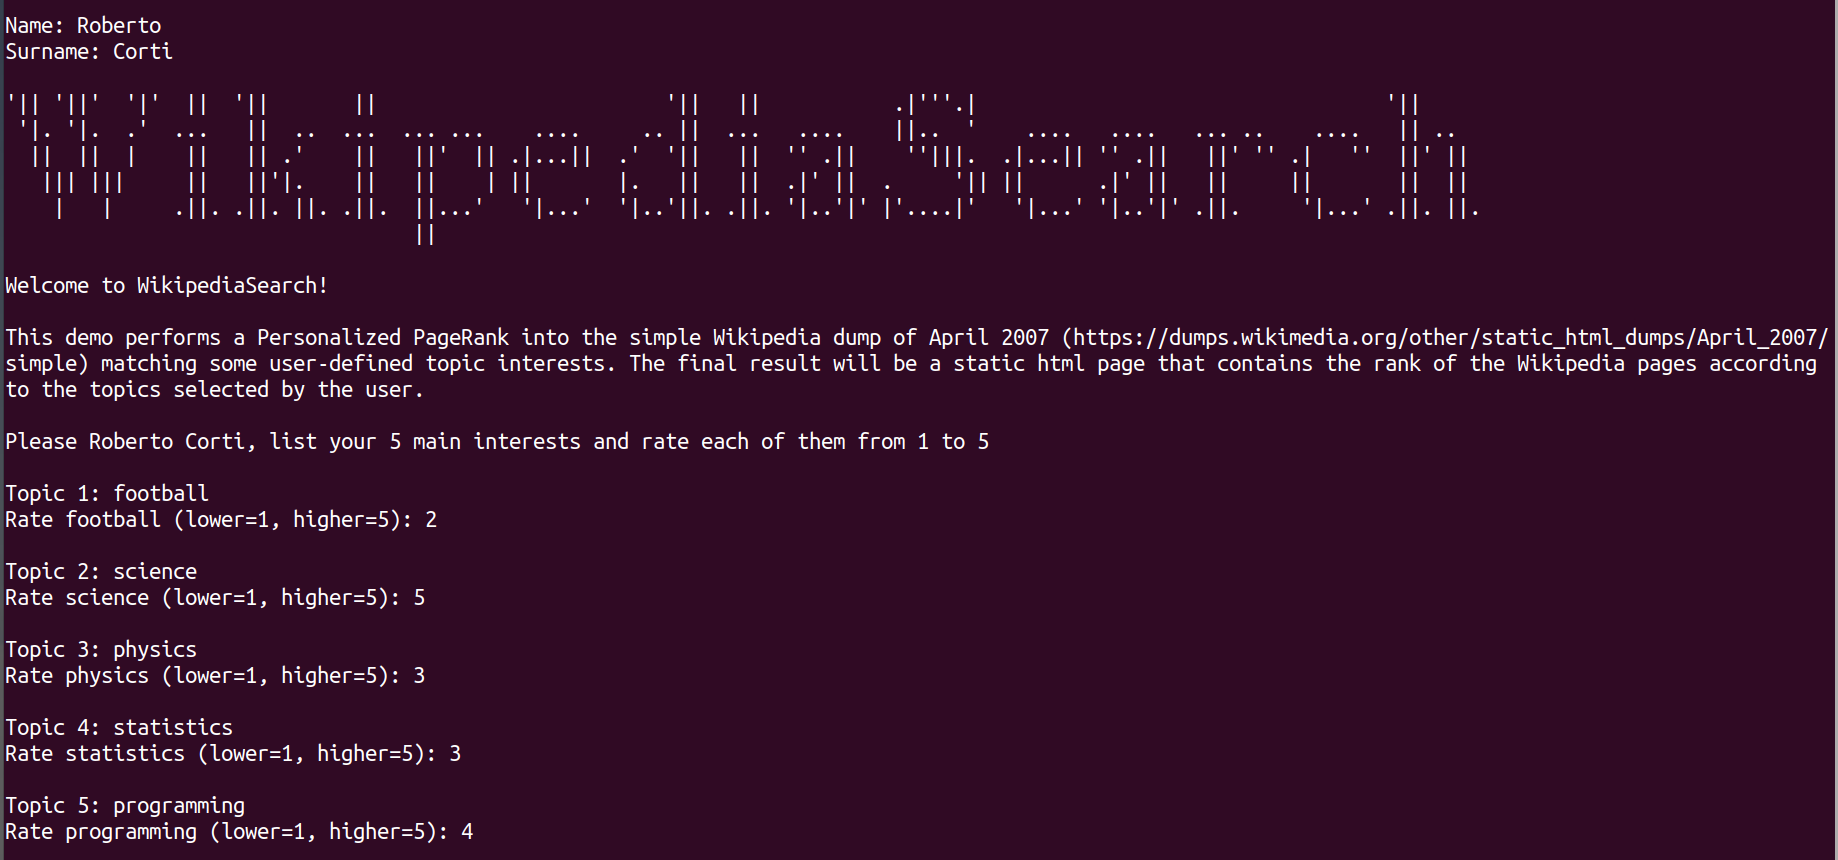
\includegraphics[scale=0.13]{input.png}
				\vspace{0.3cm}
				\caption{\textbf{Input interface}: user specifies the topics in which he/she has more interest} 
			\end{figure}  
				}
				
		\only<3>{ 
			\begin{figure}[t]
				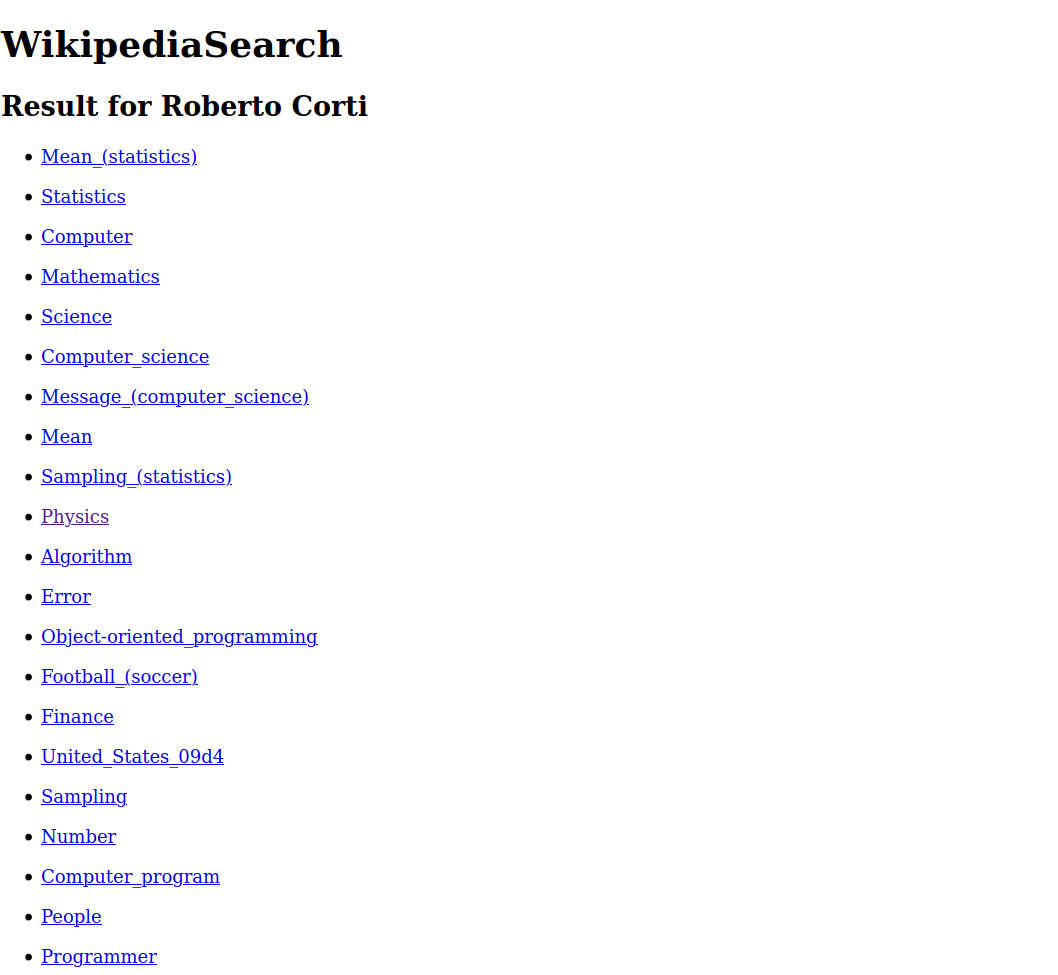
\includegraphics[scale=0.12]{output.png}
				\vspace{0.3cm}
				\caption{\textbf{Output page}: a rank of Wikipedia articles in which the user would be interested to read}
			\end{figure}  
		}
	
		
	\end{frame}
	
	\begin{frame}
		\frametitle{The problem}
		\framesubtitle{\textit{"Bringing Order to the Web"}}
	
	\end{frame}

	\begin{frame}
		\frametitle{A recap of PageRank theory}
		\framesubtitle{\textit{From L.Page and S.Brin (1998)}}
	\end{frame}
	
	
	\section{Wikipedia dataset}
	
	\begin{frame}
		\frametitle{Wikipedia ...}
		content...
	\end{frame}

	\section{WikipediaSearch implementation}
	
	\begin{frame}
		\frametitle{PageRank implementation}
	\end{frame}

	\section{WikipediaSearch evaluation}
	
	\begin{frame}
		\frametitle{Standard PageRank}
	\end{frame}
	
	\section{Conclusion}
		
	\begin{frame}
		\frametitle{Conclusion}
	\end{frame}
	
\end{document}